\section{Dimensionality Reduction}
\label{sec:dimreduce}

Using high dimensional vectors is problematic with many learning
algorithms because of computational cost and the curse of
dimensionality.  In this section we investigate if there is a low
dimensional representation of the substitute vectors which still
preserve the neighborhood information necessary to learn syntactic
categories.  We first briefly describe then report experimental
results on principal components analysis (PCA), Isomap
\cite{tenenbaum2000global}, locally linear embedding (LLE)
\cite{roweis2000nonlinear}, and Laplacian eigenmaps
\cite{belkin2003laplacian}.  

Each dimensionality reduction algorithm tries to preserve certain
aspects of the original vectors.  PCA is a linear method that
minimizes reconstruction error.  Isomap tries to preserve distances as
measured along a low dimensional submanifold assuming the input
vectors were sampled from the neighborhood of such a manifold.  LLE
most faithfully preserves the local linear structure of nearby input
vectors.  Laplacian eigenmaps most faithfully preserve proximity
relations, mapping nearby inputs to nearby outputs.

We wanted to see how accuracy (based on the k-nearest-neighbor
supervised baseline as in the previous section) changed based on the
number of dimensions for each dimensionality reduction algorithm.  All
other parameters were set empirically to values that gave reasonable
results: For algorithms that require a distance matrix rather than raw
input vectors we used the KL2 distance judged best by the experiments
of the previous section.  For graph based methods we built
neighborhood graphs using 100 nearest neighbors.  The low dimensional
output vectors were compared using the cosine distance metric for the
supervised k-nearest-neighbor algorithm.  Figure~\ref{fig:dimreduce}
plots supervised baseline accuracy vs. number of dimensions for each
algorithm.

% graph of dims vs accuracy
\begin{figure}[h]
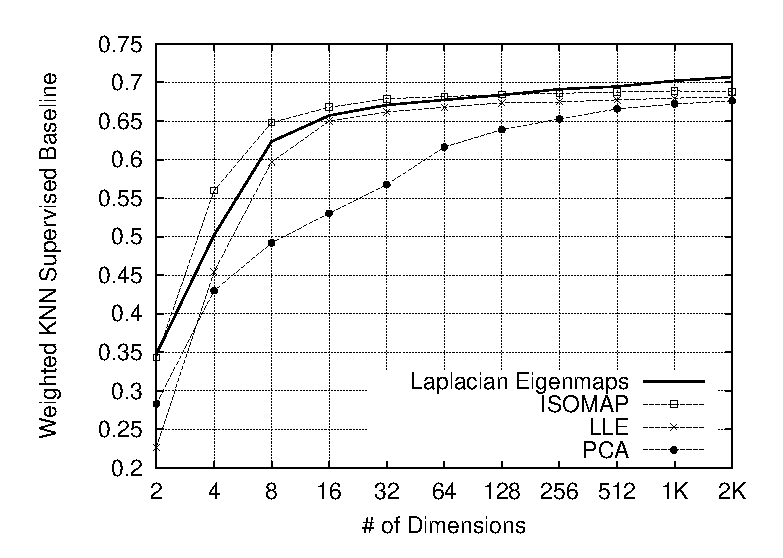
\includegraphics[width=.5\textwidth]{baseline_graph_mono.eps}
\caption{Supervised knn baselines for the four dimensionality
  reduction algorithms.}
\label{fig:dimreduce}
\end{figure}

% /scratch/esert/pos_ind/work/BASELINE_GRAPH/plot_data
% dimension PCA    LLE     ISO     LEM(Spectral)
% 2              0.2831 0.2272 0.3433 0.3480
% 4              0.4300 0.4547 0.5596 0.5019
% 8              0.4920 0.5968 0.6480 0.6234
% 16            0.5303 0.6500 0.6678 0.6572
% 32            0.5676 0.6617 0.6790 0.6708
% 64            0.6162 0.6680 0.6818 0.6774
% 128          0.6390 0.6735 0.6844 0.6838
% 256          0.6527 0.6747 0.6860 0.6914
% 512          0.6658 0.6774 0.6876 0.6948
% 1024        0.6720 0.6798 0.6891 0.7022
% 2048        0.6764 0.6811 0.6878 0.7070
% 

The graph based algorithms (Isomap, LLE, and Laplacian eigenmaps) all
outperform PCA.  They stay within 5\% of their peak accuracy with as
few as 16 dimensions.  In fact Laplacian eigenmaps outperform the
baseline with the original 12,672 dimensional vectors (68.95\%) when
allowed to retain more than about 250 dimensions.  Spectral clustering
uses the same transformation as the Laplacian eigenmaps algorithm and
we compare its performance to other clustering algorithms in the next
section.

